\documentclass{standalone}
%%%% GRAPHICS %%%%
\usepackage{tikz}
\usepackage{circuitikz}
\usetikzlibrary{arrows.meta}
\usepackage{tikz-3dplot}
\usepackage{graphicx}
\usepackage{pgfplots}
  \pgfplotsset{compat=1.18}
\usetikzlibrary{arrows}
\newcommand{\midarrow}{\tikz \draw[-triangle 90] (0,0) -- +(.1,0);}

%%%% FIGURES %%%%
\usepackage{subcaption}
\usepackage{wrapfig}
\usepackage{float}
\usepackage[skip=5pt, font=footnotesize]{caption}

%%%% FORMATTING %%%%
\usepackage{parskip}
\usepackage{tcolorbox}
\usepackage{ulem}
% \usepackage{fancyhdr}

%%%% TABLE FORMATTING %%%%
\usepackage{tabularray}
\UseTblrLibrary{booktabs}

%%%% MATH AND LOGIC %%%%
\usepackage{xifthen}
\usepackage{amsmath}
\usepackage{amssymb}
\usepackage{amsfonts}

%%%% TEXT AND SYMBOLS %%%%
\usepackage[T1]{fontenc}
\usepackage{textcomp}
\usepackage{gensymb}

%%%% OTHER %%%%
\usepackage{standalone}

%%%% LOGIC SYMBOLS %%%%
\newcommand*\xor{\oplus}

%%%% STYLES %%%%

% Packages
\usepackage{fullpage}
\usepackage{titlesec}
\usepackage[rgb]{xcolor}
\selectcolormodel{natural}
\usepackage{ninecolors}
\selectcolormodel{rgb}

% Colors
\definecolor{pg}{HTML}{24273A}
\definecolor{fg}{HTML}{FFFFFF}
\definecolor{bg}{HTML}{24273A}
\definecolor{re}{HTML}{d20f39}
\definecolor{gr}{HTML}{40a02b}
\definecolor{ye}{HTML}{df8e1d}
\definecolor{or}{HTML}{fe640b}
\definecolor{bl}{HTML}{1e66f5}
\definecolor{ma}{HTML}{8839ef}
\definecolor{cy}{HTML}{179299}
\definecolor{pi}{HTML}{ea76cb}

\usepackage{nameref}
\makeatletter
\newcommand*{\currentname}{\@currentlabelname}
\makeatother

\titleformat{\section}
  {\normalfont\scshape\Large\bfseries}
  {\thesection}
  {0.75em}
  {}

\titleformat{\subsection}
  {\normalfont\scshape\large\bfseries}
  {\thesubsection}
  {0.75em}
  {}

\titleformat{\subsubsection}
  {\normalfont\scshape\normalsize\bfseries}
  {\thesubsubsection}
  {0.75em}
  {}

% Formula
\newcounter{formula}[section]
\newenvironment{formula}[1]{
  \stepcounter{formula}
  \begin{tcolorbox}[
    standard jigsaw, % Allows opacity
    colframe={fg},
    boxrule=1px,
    colback=bg,
    opacityback=0,
    sharp corners,
    sidebyside,
    righthand width=18px,
    coltext={fg}
  ]
  \centering
  \textbf{\uline{#1}}
}{
  \tcblower
  \textbf{\thesection.\theformula}
  \end{tcolorbox}
}

% Definition
\newcounter{definition}[section]

\newenvironment{definition*}[1]{
  \begin{tcolorbox}[
    standard jigsaw, % Allows opacity
    colframe={fg},
    boxrule=1px,
    colback=bg,
    opacityback=0,
    sharp corners,
    coltext={fg}
  ]
  \textbf{#1 \hfill}
  \vspace{5px}
  \hrule
  \vspace{5px}
  \noindent
}{
  \end{tcolorbox}
}

\newenvironment{definition}[1]{
  \stepcounter{definition}
  \begin{tcolorbox}[
    standard jigsaw, % Allows opacity
    colframe={fg},
    boxrule=1px,
    colback=bg,
    opacityback=0,
    sharp corners,
    coltext={fg}
  ]
  \textbf{#1 \hfill \thesection.\thedefinition}
  \vspace{5px}
  \hrule
  \vspace{5px}
  \noindent
}{
  \end{tcolorbox}
}

% Example Problem
\newcounter{example}[section]
\newenvironment{example}{
  \stepcounter{example}
  \begin{tcolorbox}[
    standard jigsaw, % Allows opacity
    colframe={fg},
    boxrule=1px,
    colback=bg,
    opacityback=0,
    sharp corners,
    coltext={fg}
  ]
  \textbf{Example \hfill \thesection.\theexample}
  \vspace{5px}
  \hrule
  \vspace{5px}
  \noindent
}{
  \end{tcolorbox}
}

\tikzset{
  cubeBorder/.style=fg,
  cubeFilling/.style={fg!20!bg, opacity=0.25},
  gridLine/.style={very thin, gray},
  graphLine/.style={-latex, thick, fg},
}

\pgfplotsset{
  basicAxis/.style={
    grid,
    major grid style={line width=.2pt,draw=fg!50!bg},
    axis lines = box,
    axis line style = {line width = 1px},
  }
}

%%%% REFERENCES %%%%
\usepackage{hyperref}
\hypersetup{
  colorlinks  = true,
  linkcolor   = pi,
  anchorcolor = pi,
  citecolor   = pi,
  filecolor   = pi,
  menucolor   = pi,
  runcolor    = pi,
  urlcolor    = pi,
}

\author{Ethan Anthony}


\title{Figure 027}
\date{October 12, 2024}

\begin{document}
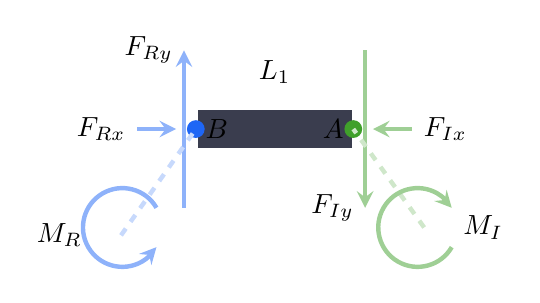
\begin{tikzpicture}

  % Beam
  \filldraw[fill=fg!10!bg, draw=fg, thick] (0,0) rectangle ++(2,0.5);

  % Wall
  \draw[draw=fg, ultra thick] (0,-1) -- ++(0,2.5);

  % F1
  % \coordinate (a) at (5,0.25);
  % \draw[draw=re, ultra thick, stealth-] (a) -- ++(0.5,1) node[anchor = south west] {$F_1$};
  % \draw[draw=fg, thick, dashed] ($(a)+(0.5,0)$) -- ++(0,1);
  % \draw[draw=fg, thick, dashed] (a) node[yshift = 5pt, xshift = 7pt] {$\theta$} -- ++(0.5,0);

  % F2
  % \coordinate (b) at (3,0.25);
  % \draw[draw=re, ultra thick, stealth-] (b) -- ++(0,1) node[anchor = south] {$F_2$};

  % B
  \coordinate (c) at (0,0.25);
  \filldraw[fill=bl, draw=bl] (c) circle (3pt) node[anchor = west] {$B$};

  % A
  \coordinate (e) at (2,0.25);
  \filldraw[fill=gr, draw=gr] (e) circle (3pt) node[anchor = east] {$A$};

  % Reaction Forces
  \draw[draw=bl!50!fg, ultra thick, stealth-] ($(c)+(-0.25,0)$) -- ++(-0.5,0) node[anchor = east] {$F_{Rx}$};
  \draw[draw=bl!50!fg, ultra thick, -stealth] ($(c)+(-0.15,-1)$) -- ++(0,2) node[anchor = east] {$F_{Ry}$};
  \coordinate (d) at (-0.5,-0.75);
  \draw[draw=bl!25!fg, ultra thick, dashed] ($(d)+(-0.45,-0.35)$) node[anchor = east, xshift = -10pt] {$M_R$} -- (c);
  \draw[-stealth,bl!50!fg, ultra thick] ($(d)+(0,0)$) arc [
    start angle = 30,
    end angle = 330,
    x radius = 0.5,
    y radius = 0.5
    ];

  % Internal Forces
  \draw[draw=gr!50!fg, ultra thick, stealth-] ($(e)+(+0.25,0)$) -- ++(0.5,0) node[anchor = west] {$F_{Ix}$};
  \draw[draw=gr!50!fg, ultra thick, stealth-] ($(e)+(0.15,-1)$) node[anchor = east] {$F_{Iy}$} -- ++(0,2);
  \draw[draw=gr!25!fg, ultra thick, dashed] ($(e)+(1.25,-1.5)+(-0.35,0.25)$) node[anchor = west, xshift = 10pt] {$M_I$} -- (e);
  \draw[-stealth,gr!50!fg, ultra thick] ($(e)+(1.25,-1.5)$) arc [
    start angle = 330,
    end angle = 30,
    x radius = 0.5,
    y radius = 0.5
    ];

  % Lengths
  \draw[draw=fg, thick, |-|] (0.1,0.7) -- node[anchor = south] {$L_1$} ++(1.8,0);
  % \draw[draw=fg, thick, |-|] (2,-0.2) -- node[anchor = north] {$L_2$} ++(1,0);
  % \draw[draw=fg, thick, |-|] (3.0,-0.2) -- node[anchor = north] {$L_3$} ++(2,0);
  % \draw[draw=fg, thick, |-|] (0.1,-0.8) -- node[anchor = north] {$L$} ++(4.9,0);
\end{tikzpicture}
\end{document}
